\section{Введение}

\section{Метод анализа колебательно-вращательной динамики.}
\subsection{Схема получения полного колебательно-вращательного гамильтониана}
\subsubsection{Переход в систему отсчета, связанную с центром масс}

\hspace{0.35cm} Рассмотрим систему $n$ материальных точек. Обозначим их массы через $m_i$, их радиус-векторы в лабораторной системе координат через $\vec{r}_i$, в подвижной системе координат -- через $\vec{R}_i$ ($i = 1 \dots n$). Разделим движение системы на движение центра масс и движение вокруг центра масс:
\vspace*{-0.1cm}
\begin{gather}
\left\{
\begin{aligned}
\vec{r}_1 &= \vec{r} + \vec{r}_1^{\ \prime}, \\
&\cdots \\
\vec{r}_n &= \vec{r} + \vec{r}_n^{\ \prime},
\end{aligned}
\right. \notag
\end{gather}

\hspace*{-0.75cm} где $\vec{r}$ -- радиус-вектор центра масс в лабораторной системе координат и $\vec{r}_i^{\ \prime}$ -- радиус-векторы рассматриваемых точек в системе отсчёта, связанной с центром масс.

Кинетическая энергия $T$ системы принимает вид: 
\vspace*{-0.1cm}
\begin{gather}
T = \frac{1}{2} \sum_{i=1}^{n} m_i \dot{\vec{r}}_i^{\ 2} = \frac{1}{2} \sum_{i=1}^{n} m_i (\dot{\vec{r}} + \dot{\vec{r}}_i^{\ \prime})^2  = \frac{1}{2} M \dot{r}^2 + \frac{1}{2} \sum_{i=1}^{n} m_i ( \dot{r}_i^\prime)^2 + \dot{\vec{r}} \sum_{i=1}^{n} m_i \dot{\vec{r}}_i^{\ \prime}, \notag
\end{gather}

\hspace*{-0.75cm} где $M = \sum_{i=1}^{n} m_i$.

Заметим, что последняя сумма является производной следующей суммы, которая равна нулю: 
\vspace*{-0.1cm}
\begin{gather}
\sum_{i=1}^{n} m_i \dot{\vec{r}}_i^{\ \prime} = \frac{d}{dt} \sum_{i=1}^{n} m_i \vec{r}_i^{\ \prime} = 0. \notag
\end{gather}

Итак, мы перешли в систему координат, связанную с центром масс, и отделили энергию движения центра масс:
\vspace*{-0.1cm}
\begin{gather}
T = \frac{1}{2} M \dot{r}^2 + \frac{1}{2} \sum_{i=1}^{n} m_i( \dot{r}_i^\prime)^2. \notag
\end{gather}

Забудем про слагаемое, отвечающее центру масс; откинем штрихи, чтобы упростить запись.

\subsubsection{Переход в подвижную систему отсчета}

Переход от лабораторной системы отсчета к подвижной системе может быть осуществлен при помощи трех последовательных поворотов на углы Эйлера $\varphi$, $\theta$ и $\psi$. 

\begin{figure}
  \centering
	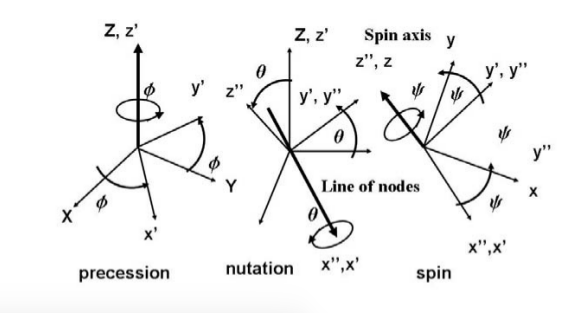
\includegraphics[width=0.7\textwidth]{../pictures/EulerAngles.jpg}
	\caption{Углы Эйлера}
	\label{fig:EulerAngles}
\end{figure}

Первое вращение происходит вокруг оси $z$ на угол $\varphi$. Оно переводит лабораторную систему $x, y, z$ в систему $x^\prime$, $y^\prime$, $z^\prime$. Угол $\varphi$ называется углом прецессии.
\begin{gather}
\begin{pmatrix}
x^\prime \\
y^\prime \\
z^\prime
\end{pmatrix} = 
\begin{pmatrix}
\cos \varphi & \sin \varphi & 0 \\
- sin \varphi & \cos \varphi & 0 \\
0 & 0 & 1
\end{pmatrix}
\begin{pmatrix}
x \\
y \\
z
\end{pmatrix} =
\bbS_\varphi
\begin{pmatrix}
x \\
y \\
z
\end{pmatrix} \notag
\end{gather}

Оси  $x^\prime$, $y^\prime$ лежат в плоскости $x$, $y$. Затем происходит поворот вокруг оси $x^\prime$ на угол $\theta$, переводящий систему $x^\prime$, $y^\prime$, $z^\prime$ в систему $x^{\dpr}$, $y^{\dpr}$, $z^{\dpr}$. Ось $x^{\dpr}$ совпадает с осью $x^{\prime}$. Ось этого поворота называется линией узлов. Угол $\theta$ называется углом нутации.

\begin{gather}
\begin{pmatrix}
x^{\dpr} \\
y^{\dpr} \\
z^{\dpr} 
\end{pmatrix} = 
\begin{pmatrix}
1 & 0 & 0 \\
0 & \cos \theta & \sin \theta \\
0 & - sin \theta & \cos \theta
\end{pmatrix}
\begin{pmatrix}
x^\prime \\
y^\prime \\
z^\prime
\end{pmatrix} = 
\bbS_\theta
\begin{pmatrix}
x^\prime \\
y^\prime \\
z^\prime
\end{pmatrix} \notag
\end{gather}   

И наконец, вращение вокруг оси $z^{\dpr}$ на угол $\psi$ переводит систему $x^{\dpr}$, $y^{\dpr}$, $z^{\dpr}$ в систему $x$, $y$, $z$. Угол $\psi$ называется углом собственного вращения.

\begin{gather}
\begin{pmatrix}
X \\
Y \\
Z
\end{pmatrix} =
\begin{pmatrix}
\cos \psi & \sin \psi & 0 \\
- \sin \psi & \cos \psi & 0 \\
0 & 0 & 1
\end{pmatrix}
\begin{pmatrix}
x^{\dpr} \\
y^{\dpr} \\
z^{\dpr}
\end{pmatrix} = 
\bbS_\psi 
\begin{pmatrix}
x^{\dpr} \\
y^{\dpr} \\
z^{\dpr}
\end{pmatrix} \notag
\end{gather}

Суммарное вращение представляет собой последовательное применение описанных поворотов и имеет следующую матрицу: 
\begin{gather}
\begin{pmatrix}
X \\
Y \\
Z
\end{pmatrix} = 
\bbS 
\begin{pmatrix}
x \\
y \\
z
\end{pmatrix} \notag \\
\bbS = \bbS_\psi \bbS_\theta \bbS_\varphi = 
\begin{pmatrix}
\cos \psi \cos \varphi - \cos \theta \sin \varphi \sin \psi & \cos \psi \sin \varphi + \cos \theta \cos \varphi \sin \psi & \sin \theta \sin \psi \\
- \sin \psi \cos \varphi - \cos \theta \sin \varphi \cos \psi & - \sin \psi \sin \varphi + \cos \theta \cos \varphi \cos \psi & \sin \theta \cos \psi \\
\sin \psi \sin \theta & - \cos \varphi \sin \theta & \cos \theta 
\end{pmatrix} \notag
\end{gather}

Проектируя вектор угловой скорости $\Omega$ на базис, образованный эйлеровыми угловыми скоростями $\dot{\varphi}$, $\dot{\theta}$, $\dot{\psi}$, получаем соотношение, известное как кинематическое уравнение Эйлера:

\begin{gather}
\begin{pmatrix}
\Omega_X \\
\Omega_Y \\
\Omega_Z
\end{pmatrix} =
\begin{pmatrix}
\sin \theta \sin \psi & \cos \psi & 0 \\
\sin \theta \cos \psi & - \sin \psi & 0 \\
\cos \theta & 0 & 1
\end{pmatrix}
\begin{pmatrix}
\dot{\varphi} \\
\dot{\theta} \\
\dot{\psi}
\end{pmatrix} \notag
\end{gather}

\begin{figure}
  \centering
	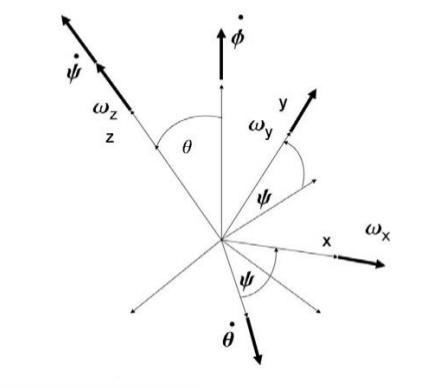
\includegraphics[width=0.5\textwidth]{../pictures/AngularVelocities.jpg}
	\caption{Угловые скорости}
	\label{fig:AngularVelocities}
\end{figure}

Перейдём в подвижную систему координат при помощи ортогональной матрицы $\bbS$:
\vverh
\begin{gather}
\vec{r}_i = \bbS \vec{R}_i, \quad i = 1 \dots n. \notag
\end{gather}

Введем матрицу $\bbA$ следующим образом: $\bbA = \dot{\bbS} \bbS^{-1}$. Покажем, что она является кососимметрической матрицей; для этого продифференцируем единичную матрицу:
\vverh
\begin{gather}
\frac{d}{dt} \bbE = \frac{d}{dt} \left( \bbS \bbS^{-1}\right) = \dot{\bbS} \bbS^{-1} + \bbS \dot{\bbS}^{-1} = 0. \notag
\end{gather}

Заметим, что первое слагаемое и есть матрица $\bbA$, а второе -- транспонированная матрица $\bbA$ (т.к. $\bbS^\top = \bbS^{-1}$ в силу ортогональности). Следовательно,
\vverh
\begin{gather}
\bbA + \bbA^\top = 0, \notag
\end{gather}

\hspace*{-0.75cm} т.е. по определению матрица $\bbA$ является кососимметрической.

Так как размерность пространства кососимметрических матриц равна 3, то существует естественный изоморфизм, позволяющий сопоставить каждой кососимметрической матрице единственный псевдовектор:
\vverh
\begin{gather}
\bbA = 
\begin{pmatrix}
0 & -\omega_3 & \omega_2 \\
\omega_3 & 0 & -\omega_1 \\
-\omega_2 & \omega_1 & 0
\end{pmatrix}
\quad
\longleftrightarrow
\quad
\vec{\omega} = 
\begin{pmatrix}
\omega_1 \\
\omega_2 \\
\omega_3
\end{pmatrix}
,
\notag
\end{gather}

\hspace*{-0.75cm} причем для любого вектора $\vec{x} \in \mathbf{R}^3$ имеем $\bbA \vec{x} = [ \vec{\omega} \times \vec{x} ]$, где $\vec{\omega}$ -- вектор угловой скорости в лабораторной системе координат.

Получим выражение для квадратов скоростей рассматриваемых точек в лабораторной системе координат через координаты и скорости в подвижной системе координат:
\vverh
\begin{gather}
\dot{\vec{r}}_i = \bbS \dot{\vec{R}}_i + \dot{\bbS} \vec{R}_i = \dot{\bbS} \bbS^{-1} \vec{r}_i + \bbS \dot{\vec{R}}_i  = \bbA \vec{r}_i + \bbS \dot{\vec{R}}_i = [ \vec{\omega} \times \vec{r}_i ] + \bbS \dot{\vec{R}}_i = [\bbS \vec{\Omega} \times \bbS \vec{R}_i ] + \bbS \dot{\vec{R}}_i = \notag \\
= \bbS \left( [\vec{\Omega} \times \vec{R}_i ] + \dot{\vec{R}}_i \right)  \notag , \\
\dot{r}_i^2 = \dot{\vec{r}}_i^{\ \top} \dot{\vec{r}}_i = \left( \dot{\vec{R}}_i + [ \vec{\Omega} \times \vec{R}_i] \right)^\top \bbS^\top \bbS \left( \dot{\vec{R}}_i + [ \vec{\Omega} \times \vec{R}_i ] \right) = \dot{R}_i^2 + 2 \dot{\vec{R}}_i \ [ \vec{\Omega} \times \vec{R}_i] + [ \vec{\Omega} \times \vec{R}_i ]^2 \notag ,
\end{gather}

\hspace*{-0.75cm} где $\vec{\Omega}$ -- вектор угловой скорости в подвижной системе координат.

Рассмотрим последнее слагаемое как смешанное произведение и применим правило Лагранжа:
\vverh
\begin{gather}
([\vec{\Omega} \times \vec{R}_i] , [\vec{\Omega} \times \vec{R}_i]) = \vec{\Omega}^\top [ \vec{R}_i \times [ \vec{\Omega} \times \vec{R}_i ]] = \vec{\Omega}^\top \left( \vec{\Omega} (\vec{R}_i, \vec{R}_i ) - \vec{R}_i (\vec{R}_i, \vec{\Omega} ) \right)
\notag .
\end{gather}

Итак, с учётом выполненных преобразований имеем:
\vverh
\begin{gather}
T = \frac{1}{2} \sum_{i=1}^{n} m_i \dot{r}_i^2 = \frac{1}{2} \sum_{i=1}^{n} m_i \dot{R}_i^2 + \vec{\Omega} ^\top \sum_{i=1}^{n} m_i[ \vec{R}_i \times \dot{\vec{R}}_i ] + \frac{1}{2} \vec{\Omega}^\top \sum_{i=1}^{n} m_i \left( \vec{\Omega} (\vec{R}_i, \vec{R}_i ) - \vec{R}_i (\vec{R}_i, \vec{\Omega} ) \right) = 
\notag \\
= \frac{1}{2} \sum_{i=1}^{n} m_i \dot{R}_i^2 + \vec{\Omega}^\top \sum_{i=1}^{n} m_i [ \vec{R}_i \times \dot{\vec{R}}_i ] + \vec{\Omega}^\top \mathbb{I} \ \vec{\Omega} \notag .
\end{gather}

\vlevo где $\bbI$ -- матрица тензора инерции в подвижной системе координат.

Пусть исследуемая система содержит $s$ внутренних степеней свободы. Осуществим переход от векторов в подвижной системе к внутренним координатам $q_j, j=1 \dots s$:
\vverh
\begin{gather}
\left\{
\begin{aligned}
\vec{R}_1 &= \vec{R}_1 (q_1, \dots, q_s), \\
&\cdots \\
\vec{R}_n &= \vec{R}_n (q_1, \dots, q_s);
\end{aligned}
\right. \notag \\
\frac{d}{dt} \vec{R}_i = \sum_{j=1}^{s} \frac{\partial \vec{R}_i}{\partial q_j} \ \dot{q}_j \notag .
\end{gather}

Подставляя $\dot{\vec{R}}_i$ в выражение для кинетической энергии, получим:
\vverh
\begin{gather}
T = \frac{1}{2} \sum_{i=1}^{n} m_i \sum_{j=1}^{s} \frac{\partial \vec{R}_i}{\partial q_j} \dot{q}_j \sum_{k=1}^{s} \frac{\partial \vec{R}_i}{\partial q_k} \dot{q}_k + \vec{\Omega}^\top \sum_{i=1}^{n} m_i \left[ \vec{R}_i \times \sum_{j=1}^{s} \frac{\partial \vec{R}_i}{\partial q_j} \ \dot{q}_j \right] + \vec{\Omega}^\top \bbI \ \vec{\Omega} = \notag \\
= \frac{1}{2} \sum_{j=1}^{s} \sum_{k=1}^{s} \left( \sum_{i=1}^{n} m_i \frac{\partial \vec{R}_i}{\partial q_j} \frac{\partial \vec{R}_i}{\partial q_k} \right) \dot{q}_j \dot{q}_k + \vec{\Omega}^\top \sum_{j=1}^{s} \left( \sum_{i=1}^{n} m_i \left[ \vec{R}_i \times \frac{\partial \vec{R}_i}{\partial q_j} \right] \right) \dot{q}_j + \frac{1}{2} \vec{\Omega}^\top \bbI \ \vec{\Omega} \notag .
\end{gather}

Обозначая $a_{jk} = \sum_{i=1}^{n} m_i \frac{\partial \vec{R}_i}{\partial q_j} \frac{\partial \vec{R}_i}{\partial q_k}$, $A_{jk} = \sum_{i=1}^{n} m_i \left[ \vec{R}_i \times \frac{\partial \vec{R}_i}{\partial q_k} \right]_{\alpha}$ (здесь $\alpha = x,y,z$ соответствуют $j=1,2,3$), представим кинетическую энергию в виде:
\vverh
\begin{gather}
T = \frac{1}{2} \dot{\vec{q}}^{\, \top} \bba \ \dot{\vec{q}} + \vec{\Omega}^\top \bbA \ \dot{\vec{q}} + \frac{1}{2} \vec{\Omega}^\top \bbI \ \vec{\Omega} \notag ,
\end{gather}

\vlevo где $\bba = (a_{jk})_{j=1 \dots s, \ k=1 \dots s}$, $\bbA = (A_{jk})_{j=1 \dots 3, \ k=1 \dots s}$.

Несложно заметить, что матрица $\bba$ является симметричной: $\bba = \bba^{\top}$.

\subsubsection{Применение теоремы Донкина}
Перепишем выражение для кинетической энергии в матричном виде для того, чтобы перейти к гамильтоновым переменным.
\begin{gather}
T = \frac{1}{2} 
\begin{bmatrix}
\vec{\Omega}^{\top} \ \dot{\vec{q}}^{\, \top}
\end{bmatrix}
\bbB
\begin{bmatrix}
\vec{\Omega} \\
\dot{\vec{q}}
\end{bmatrix}, \notag
\end{gather}

где $\bbB$ -- блочная матрица:
\begin{gather}
\bbB = 
\begin{bmatrix}
\bbI & \bbA \\
\bbA^{\dn \top} & \bba
\end{bmatrix} \notag
\end{gather}  

\begin{minipage}[c]{0.55\linewidth}
\begin{tikzpicture}[framed]

  \tikzstyle{arrow} = [thick, ->, >=stealth]
\tikzstyle{vecArrow} = [thick, decoration={markings,mark=at position
   1 with {\arrow[semithick]{open triangle 60}}},
   double distance=1.4pt, shorten >= 5.5pt,
   preaction = {decorate},
   postaction = {draw,line width=1.4pt, white,shorten >= 4.5pt}]

\tikzstyle{lagrange} = [rectangle, rounded corners, minimum width = 3cm, minimum height = 1cm, text centered, text width = 7cm, draw = black, fill=red!30]

\tikzstyle{hamilton} = [rectangle, rounded corners, minimum width = 3cm, minimum height = 1cm, text centered, text width = 7cm, draw = black, fill=yellow!30]

\tikzstyle{equations} = [rectangle, rounded corners, minimum width = 3cm, minimum height = 1cm, text centered, text width = 5cm, draw = black, fill=green!30]
    
\begin{tikzpicture}[node distance = 2cm, auto]

\node (lag1) [lagrange] {$\mathcal{L} = \mathcal{L}(\vec{q}, \dot{\vec{q}})$};

\node (ham1) [hamilton, right = 2 cm of lag1] {$\mathcal{H} = \mathcal{H}(\vec{q}, \vec{p})$};

\node (eq1) [equations, below = 0.5 cm of lag1] {$\vec{p} = \frac{\partial \mathcal{L}}{\partial \dot{\vec{q}}}$};

\node (eq2) [equations, below = 0.5 cm of ham1] {$\dot{\vec{q}} = \frac{\partial \mathcal{L}}{\partial \vec{p}}$};

\node (lag2) [lagrange, below = 2 cm of lag1] {$\mathcal{L} = \mathcal{L}(\vec{\Omega})$};

\node (ham2) [hamilton, below = 2 cm of ham1] {$\mathcal{H} = \mathcal{H} (\vec{J})$};

\node (eq3) [equations, below = 0.5 cm of lag2] {$\vec{J} = \frac{\partial \mathcal{L}}{\partial \vec{\Omega}}$};

\node (eq4) [equations, below = 0.5 cm of ham2] {$\vec{\Omega} = \frac{\partial \mathcal{H}}{\partial \vec{J}}$};

\draw [vecArrow] (lag1) -- (ham1);

\draw [vecArrow] (lag2) -- (ham2);

\end{tikzpicture}


 
  \begin{scope}[on background layer]
    \node [fill=black!30,fit= (lag1) (lag2) (ham1) (ham2) (eq1) (eq2) (eq3) (eq4)] {};
  \end{scope}

\end{tikzpicture}
\end{minipage}
\begin{minipage}[c]{0.4\linewidth}
Текст, поясняющий, что угловая скорость и угловой момент являются такими же сопряженными переменными как $\vec{q}$ и $\vec{p}$.
\end{minipage} \\

Сейчас мы работаем исключительно с выражением для кинетической энергии, так что обозначим имеющееся у нас выражение $T_\mathcal{L}$ (в лагранжевом представлении), а искомое представление -- $T_\mathcal{H}$.
\vverh
\begin{gather}
\vec{p} = \frac{\partial T_\mathcal{L}}{\partial \dot{\vec{q}}} = \bbA^{\dn \top} \vec{\Omega} + \bba \dot{\vec{q}} \notag \\
\vec{J} = \frac{\partial T_\mathcal{L}}{\partial \vec{\Omega}} = \bbI \, \vec{\Omega} + \bbA \dot{\vec{q}} \notag
\end{gather}

Заметим, что блочный вектор $\begin{bmatrix} \vec{J} \\ \vec{p} \end{bmatrix}$ связан с вектором $\begin{bmatrix} \vec{\Omega} \\ \dot{\vec{q}} \end{bmatrix}$ линейным преобразованием, причем матрица этого линейного преобразования есть $\bbB$:
\vverh
\begin{gather}
\begin{bmatrix}
\vec{J} \\
\vec{p}
\end{bmatrix}
= \bbB
\begin{bmatrix}
\vec{\Omega} \\
\dot{\vec{q}}
\end{bmatrix}
\quad \implies \quad 
\begin{bmatrix}
\vec{\Omega} \\
\dot{\vec{q}}
\end{bmatrix}
= \bbB^{-1}
\begin{bmatrix}
\vec{J} \\
\vec{p}
\end{bmatrix} \notag
\end{gather}

Инвертирование блочной матрицы $\bbB$ легче всего осуществить с применением формул Фробениуса. (Аппендикс \ref{appendix:frobenius}).
Обозначим $\bbG = \bbB^{-1} = \begin{bmatrix} G_{11} & G_{12} \\ G_{21} & G_{22}
\end{bmatrix}$, ее элементы имеют следующие выражения:
\vverh
\begin{gather}
\begin{aligned}
\bbG_{11} &=  \lb \bbI - \bbA \bba^{-1} \bbA^{\dn \top} \rb^{-1} \\
\bbG_{12} &= - \bbI^{-1} \bbA \bbG_{22} = - \bbG_{11} \bbA \bba^{-1}\\
\bbG_{21} &= - \bba^{-1} \bbA^{\dn \top} \bbG_{11} = \bbG_{22} \bbA^{\dn \top} \bbI^{-1} \\
\bbG_{22} &= \lb \bba - \bbA^{\dn \top} \bbI^{-1} \bbA \rb^{-1}.
\end{aligned}
\notag
\end{gather}

Легко заметить, что $\bbG_{12} = \bbG_{21}^{\top}$. Используем этот факт в ходе стандартной процедуры перехода к гамильтоновому представлению кинетической энергии.
\vverh
\begin{gather}
\begin{bmatrix}
\vec{\Omega} \ \\
\dot{\vec{q}} 
\end{bmatrix}
= \bbG
\begin{bmatrix}
\vec{J} \ \\
\vec{p}
\end{bmatrix}
\quad \implies \quad
\begin{bmatrix}
\vec{\Omega}^{\top} \ \dot{\vec{q}}^{\, \top}
\end{bmatrix}
= 
\begin{bmatrix}
\vec{J}^{\, \top} \ \vec{p}^{\, \top}
\end{bmatrix}
\bbG \notag \\
T_\mathcal{H} = 
\begin{bmatrix}
\vec{\Omega}^{\top} \ \dot{\vec{q}}^{\, \top}
\end{bmatrix}
\begin{bmatrix}
\vec{J} \ \\
\vec{p}
\end{bmatrix} 
- T_\mathcal{L} = \frac{1}{2} 
\begin{bmatrix}
\vec{J}^{\, \top} \ \vec{p}^{\, \top}
\end{bmatrix} 
\bbG
\begin{bmatrix}
\vec{J} \ \\
\vec{p}
\end{bmatrix} = 
\frac{1}{2} \vec{J}^{\, \top} \bbG_{11} \vec{J} + \frac{1}{2} \, \vec{p}^{\, \top} \bbG_{22} \, \vec{p} + \vec{J}^{\, \top} \bbG_{12} \, \vec{p} \notag
\end{gather}

\subsection{Обобщенные уравнения Эйлера}
В изолированной системе в лабораторной системе координат, связанной с центром масс системы, угловой момент является интегралом движения: $\dot{\vec{j}} = 0$. Векторы углового момента в подвижной системе координат и в лаборатной системе координат будут связаны следующим соотношением: 
\vverh
\begin{gather}
\vec{J} = \bbS \vec{j}. \label{j1}
\end{gather} 

Переписывая это соотношение через угловую скорость $\vec{\Omega}$ подвижной системы отсчета относительно лабораторной системы (в проекции на подвижную систему отсчета), получаем:
\vverh
\begin{gather}
\dot{\vec{J}} + \left[ \vec{\Omega} \times \vec{J} \right] = \vec{0} \label{j2}
\end{gather}

Согласно теореме Донкина, имеем: $\vec{\Omega} = \partial \mathcal{H} / \partial \vec{J}$. Модифицируя уравнение \eqref{j2} согласно утверждению теоремы Донкина, приходим к системе уравнений, которую будем называть \textit{обобщенными уравнениями Эйлера}.
\vverh
\begin{gather}
\dot{\vec{J}} + \left[ \frac{\partial \mathcal{H}}{\partial \vec{J}} \times \vec{J} \right] = \vec{0} \notag
\end{gather}

Возвращаясь к связи между векторами углового момента в подвижной и лабораторной системах отсчета \eqref{j1}, заметим, что $J = | \vec{J} |$ - модуль вектора углового момента является интегралом движения. Это позволит использовать только два из трех обобщенных уравнений Эйлера. Введем угловые переменные $\Theta$ и $\Phi$, определяющие направление вектора углового момента $\vec{J}$ в подвижной системе отсчета:
\vverh
\begin{gather}
\left\{
\begin{aligned}
J_x &= J \sin \Theta \cos \Phi \\
J_y &= J \sin \Theta \sin \Phi \\
J_z &= J \cos \Theta
\end{aligned}
\right. \notag
\end{gather}

\iffalse
Дифференцируя компоненты углового момента по сферическим углам $\Theta$ и $\Phi$, получаем:
\vverh
\begin{gather}
\left\{
\begin{aligned}
\dot{J}_x &= - \dot{\Phi} J \sin \Phi \sin \Theta + \dot{\Theta} J \cos \Phi \cos \Theta \\
\dot{J}_y &= \dot{\Phi} J \cos \Phi \sin \Theta + \dot{\Theta} J \sin \Phi \cos \Theta \\
\dot{J}_z &= - \dot{\Theta} J \sin \Theta
\end{aligned}
\right.\notag
\end{gather}
\fi

Выражаем $\dot{\Phi}$ как линейную комбинацию $\dot{J}_x$, $\dot{J}_y$; $\dot{\Theta}$ -- через $\dot{J}_z$, подставляем выражения производных компонентов углового момента из обобщенных уравнений Эйлера. 
\vverh
\begin{gather}
\left\{
\begin{aligned}
\dot{\Phi} &= \lb \frac{\partial \mathcal{H}}{\partial J_x} \cos \Phi + \frac{\partial \mathcal{H}}{\partial J_y} \sin \Phi \rb \ctg \Theta - \frac{\partial \mathcal{H}}{\partial J_z} \\
\dot{\Theta} &= \frac{\partial \mathcal{H}}{\partial J_x} \sin \Phi - \frac{\partial \mathcal{H}}{\partial J_y} \cos \Phi 
\end{aligned}
\right. \notag
\end{gather}

\subsection{Полная система динамических уравнений.}

Подводя итог предыдущим выкладкам, определен метод получения точного колебательно-вращательного гамильтониана $\mathcal{H} = \mathcal{H} (\vec{q}, \vec{p}, \vec{J})$. Полная система динамических уравнений может быть представлена в следующей форме:
\vverh
\begin{gather}
\left\{
\begin{aligned}
\dot{\vec{q}} &= \frac{\partial \mathcal{H}}{\partial \vec{p}} \\
\dot{\vec{p}} &= - \frac{\partial \mathcal{H}}{\partial \vec{q}} \\
\dot{\vec{J}} &+ \left[ \frac{\partial \mathcal{H}}{\partial \vec{J}} \times \vec{J} \right] = \vec{0}  
\end{aligned}
\right.
\quad \implies \quad
\left\{
\begin{aligned}
\dot{\Phi} &= \lb \frac{\partial \mathcal{H}}{\partial J_x} \cos \Phi + \frac{\partial \mathcal{H}}{\partial J_y} \sin \Phi \rb \ctg \Theta - \frac{\partial \mathcal{H}}{\partial J_z} \\
\dot{\Theta} &= \frac{\partial \mathcal{H}}{\partial J_x} \sin \Phi - \frac{\partial \mathcal{H}}{\partial J_y} \cos \Phi \\
\dot{\vec{q}} &= \frac{\partial \mathcal{H}}{\partial \vec{p}} \\
\dot{\vec{p}} &= - \frac{\partial \mathcal{H}}{\partial \vec{q}}
\end{aligned},
\right. \label{total_sys}
\end{gather}

\vlevo где $\partial \mathcal{H} / \partial J_\alpha = \partial \mathcal{H} / \partial J_\alpha (\vec{q}, \vec{p}, \Theta, \Phi)$, $\alpha = x,y,z$.

Углы $\Theta$, $\Phi$ описывают двумерное подпространство вращательной задачи в $(2s+2)$-мерном фазовом пространстве колебательно-вращательной задачи. В результате решения системы дифференциальных уравнений \eqref{total_sys} имеем зависимости $\Theta = \Theta(t)$, $\Phi = \Phi(t)$, которые параметрически задают вращательную фазовую траекторию -- траекторию конца вектора углового момента $\vec{J}$ на сфере радиуса $J$.\\
Необходимо отметить, что для произвольной системы с $s$ внутренними степенями свободы система \eqref{total_sys} содержит минимально возможное количество динамических уравнений, $2s+2$. Т.е. заданные интегралы движения колебательно-вращательной задачи в максимальной степени учтены при формировании системы динамических уравнений \eqref{total_sys}. Это свойство качественно отличает описанный подход от традиционно применяемых способов расчета классических траекторий, количество уравнений в которых заведомо больше необходимого, а контроль за сохранением энергии и углового момента осуществляется лишь численно. 

\hspace*{-1cm}
\begin{tikzpicture}[framed]

  \tikzstyle{lagrange} = [rectangle, rounded corners, minimum width = 3cm, minimum height = 1cm, text centered, text width = 7cm, draw = black, fill=red!30]

\tikzstyle{hamilton} = [rectangle, rounded corners, minimum width = 3cm, minimum height = 1cm, text centered, text width = 7cm, draw = black, fill=yellow!30]

\tikzstyle{equations} = [rectangle, rounded corners, minimum width = 3cm, minimum height = 1cm, text centered, text width = 5cm, draw = black, fill=green!30]

\tikzstyle{equations_big} = [rectangle, rounded corners, minimum width = 3cm, minimum height = 1cm, text centered, text width = 8cm ,draw = black, fill = green!30]

\tikzstyle{arrow} = [thick, ->, >=stealth]
\tikzstyle{arrow_comes_above} = [thick, ->, >=stealth, yshift=10pt]

\tikzstyle{vecArrow} = [thick, decoration={markings,mark=at position
   1 with {\arrow[semithick]{open triangle 60}}},
   double distance=1.4pt, shorten >= 5.5pt,
   preaction = {decorate},
   postaction = {draw,line width=1.4pt, white,shorten >= 4.5pt}]

\node (lag1) [lagrange] {$\mathcal{L} = \mathcal{L}(\vec{r}_1^{\ \prime},  \cdots, \vec{r}_n^{\ \prime}, \dot{\vec{r}}_1^{\ \prime}, \cdots, \dot{\vec{r}}_n^{\ \prime})$};

\node (lag2) [lagrange, below = 1.5 cm of lag1] {$\mathcal{L} = \mathcal{L} (\vec{r}_1, \cdots, \vec{r}_{n-1}, \dot{\vec{r}}_1, \cdots, \dot{\vec{r}}_{n-1})$};

\node (lag3) [lagrange, below = 1.5 cm of lag2] {$\mathcal{L} = \mathcal{L}(\vec{R}_1, \cdots, \vec{R}_n, \dot{\vec{R}}_1, \cdots, \dot{\vec{R}}_{n-1}, \vec{\Omega})$};

\node (lag4) [lagrange, below = 1.5 cm of lag3] {$\mathcal{L} = \mathcal{L}(\vec{q}_1, \cdots, \vec{q}_s, \dot{\vec{q}}_1, \cdots, \dot{\vec{q}}_s, \vec{\Omega})$};

\node (ham1) [hamilton, below = 2.5 cm of lag4] {$\mathcal{H} = \mathcal{H}(\vec{q}_1, \cdots, \vec{q}_s, \vec{p}_1, \cdots, \vec{p}_s, \vec{J})$};

\node (eq1) [equations, below right = 0.1cm and 1cm of lag1] {$
\vec{r}_i^{\ \prime} = \vec{R} + \vec{r}_i 
$};

\node (eq2) [equations, below right = 0.2cm and 1cm of lag2] {$
\vec{r}_i = \mathbb{S} \vec{R}_i
$};

\node (eq3) [equations, below right = 0.0cm and 1cm of lag3] {$
\vec{R}_i = \vec{R}_i(q_1, \cdots, q_s)
$};

\node (eq4) [equations, below right = 0.0cm and 1cm of lag4] {$
\left\{
\begin{aligned}
J &= \frac{\partial \mathcal{L}}{\partial \Omega} \\
p &= \frac{\partial \mathcal{L}}{\partial \dot{q}}
\end{aligned}
\right.
$};

\node (eq5) [equations, below left = 1.5 cm and 0.1 cm of ham1] {$
\left\{
\begin{aligned}
\dot{\vec{p}} &= \frac{\partial \mathcal{H}}{\partial \vec{q}} \\
\dot{\vec{q}} &= - \frac{\partial \mathcal{H}}{\partial \vec{p}} \\
\dot{\vec{J}} &+ [ \frac{\partial \mathcal{H}}{\partial \vec{J}} \times \vec{J} ] = 0 
\end{aligned}
\right.
$};

\node (eq6) [equations_big, right = 3 cm of eq5] {$
\left\{
\begin{aligned}
\dot{\vec{p}} &= \frac{\partial \mathcal{H}}{\partial \vec{q}} \\
\dot{\vec{q}} &= - \frac{\partial \mathcal{H}}{\partial \vec{p}} \\
\dot{\varphi} &= \left( \frac{\partial \mathcal{H}}{\partial J_x} \cos \varphi + \frac{\partial \mathcal{H}}{\partial J_y} \sin \varphi \right) \ctg \theta - \frac{\partial \mathcal{H}}{\partial J_z} \\
\dot{\theta} &= \frac{\partial \mathcal{H}}{\partial J_x} \sin \varphi - \frac{\partial \mathcal{H}}{\partial J_y} \cos \varphi
\end{aligned}
\right.
$};

\draw [vecArrow] (lag1) -- node[anchor = east] {Transition to COM-frame} (lag2);
\draw [vecArrow] (lag2) -- node[anchor = east] {Transition to rotating frame} (lag3);
\draw [vecArrow] (lag3) -- node[anchor = east] {Transition to internal coordinates} (lag4);
\draw [vecArrow] (lag4) -- node[anchor = east] {Legendre transformation} (ham1);
\draw [vecArrow] (ham1) -| (eq5);
\draw [vecArrow] (eq5) -- (eq6);

\draw [arrow] (lag1) -| (eq1);
\draw [arrow_comes_above] (eq1) |- ([yshift=10pt]lag2);
\draw [arrow] ([yshift=-10pt]lag2) -| (eq2);
\draw [arrow_comes_above] (eq2) |- ([yshift=10pt]lag3);
\draw [arrow] ([yshift=-10pt]lag3) -| (eq3);
\draw [arrow_comes_above] (eq3) |- ([yshift=10pt]lag4);
\draw [arrow] ([yshift=-10pt]lag4) -| (eq4);
\draw [arrow_comes_above] (eq4) |- (ham1);
 
  \begin{scope}[on background layer]
    \node [fill=black!30,fit= (lag1) (lag2) (lag3) (lag4) (ham1) (eq1) (eq2) (eq3) (eq4) (eq5) (eq6)] {};
  \end{scope}

\end{tikzpicture}

